
La dependencia de los combustibles fósiles traería consigo problemas como la inseguridad energética y el incremento de la temperatura global a causa del aumento de los gases de efecto invernadero. Las sociedades que concentran la producción de los combustibles fósiles podrían controlar geopolítica y económicamente a otras \cite{mayer2022fossil}, esta inseguridad energética se evidenció en la crísis del petróleo de 1973 \cite{vernon1976oil} y en la disputa entre Rusia y la Unión Europea por el suministro de gas en este año \cite{rodriguez2022improving}. En contraste, el problema del incremento de la temperatura global es un problema mediáticamente más discreto pero no menos alarmante. Tanto así que, en el 2018, la \textit{Intergovernmental Panel on Climate Change} (IPCC) emitió un informe sobre los impactos que causaría dicho incremento en 1.5°C con respecto a los niveles preindustriales para el 2040, que en resumidas cuentas, se prevé un detrimento crítico y sin retorno de la civilización y la biósfera \cite{guilyardi2018ipcc}. A fin de hacer frente a estos problemas, la transición hacia una matriz energética mundial donde predominen fuentes energéticas menos contaminantes y descentralizadas es la solución. 



Las fuentes renovables reunen dichas características, por lo que muchos gobiernos y organizaciones han tomado acciones para aprovecharlas. En ese marco, la \textit{International Renewable Energy Agency} (IRENA) realizó un análisis multisectorial en el 2020 donde propuso una hoja de ruta para que las energías renovables generen el 86\% de la electricidad global \cite{asmelash2020role}. En ese documento también se menciona que esta cifra no se alcanzaría sin la investigación ni el desarrollo de tecnologías que aprovechen dichas fuentes para hacerlas sostenibles y comercialmente viables.

\begin{figure}[!ht]
    \begin{center}
        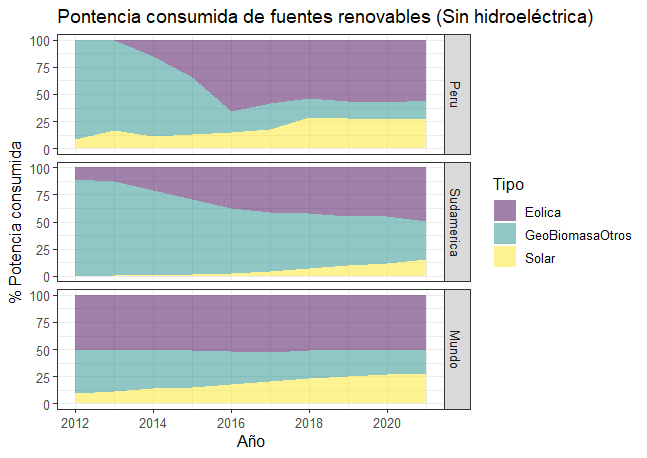
\includegraphics[scale=0.80]{img/PorcentajeRenovable.png}
    \end{center}
    \caption{Comparación del porcentaje de la cantidad de potencia consumida por tipo de energía renovable sin considerar la hidroeléctrica.
    Fuente: Our World in Data \cite{owidenergy}}
    \label{img:PorcentajeRenovable}
\end{figure}

Hace un año, la energía hidroeléctrica generó más de 4 mil tera-vatios por hora (TWh) en el mundo, lo que representó más del 50\% de la generación de todas las renovables \cite{irena2022international}. No obstante, no es posible extender la construcción de centrales hidroeléctricas dado que muchas comunidades no cuentan cuencas hidrográficas o caídas de agua que puedan aprovecharse. Sin contar esta fuente, las energías eólica y solar son las que encabezan la producción energética. Con el propósito de contextualizar el crecimiento del uso de estas fuentes renovables geográfica y temporalmente se muestra la Figura \ref{img:PorcentajeRenovable}. En ella se visualizan los porcentajes de potencia consumida provenientes de tres grupos de fuentes renovables no hídroeléctricas: La eólica, solar y otras (\textit{GeoBiomasaOtros}). Estos porcentajes se distribuyen desde el 2012 hasta el 2021 y se comparan las tendencias en el Perú, Sudamérica y el mundo. Se aprecia el aumento del consumo energético de la eólica y solar sobre las demás, y de entre estas dos, la eólica es mayor. No obstante, también es evidente que la energía solar ha tenido un crecimiento sostenido en el tiempo y esto se debe, entre otras razones, a la disponibilidad de nuevas tecnologías más comercial y ambientalmente más viables que aprovechan la luz solar.



Existen dos tipos de tecnlogías solares: La termosolar y la fotovoltaica \cite{hammarstrom2012}. En la primera se usa la energía térmica de un fluído calentado por concentradores solares para generar electricidad por medio del movimiento de turbinas contectadas a generadores electromagnéticos. Pese a los esfuerzos por reducir los costos de construcción y mantenimiento de las centrales termosolares, solo países con alta demanda energética industrial y la geografía apta pueden hacer rentables estas tecnologías \cite{xu2022concentrated}.


En contraste a la termosolar, en la fotovoltaica se aprovecha directamente la radiación solar mediante fenómenos fotoeléctricos y de transporte de cargas, mimetizando la fotosíntesis. Si las plantas tienen a las células con clorofila en sus hojas como sus unidades generadoras de energía, en los sistemas fotovoltaicos estas serían las células o celdas solares. La estructura de una celda solar depende de los mecanismos de generación eléctrica y trasporte de carga, y estos a su vez, de la naturaleza de los materiales donde suceden estos mecanismos. El interés por desarrollar tecnologías fotovoltaicas se da por dos razones: Por su versatilidad, es decir que pueden ser usadas para fines domésticos o industriales, y  porque reducirían notablemente las emisiones de $CO_2$/kWh, por ejemplo esta reducción sería cercana al 90\% para sistemas que sustituyan al gas natural \cite{tawalbeh2021environmental}.


Las celdas solares llevan en el mercado más de 60 años, desde su descubrimiento en los  Laboratorios Bell en 1954 \cite{green2009path} y su primer uso comercial en el satélite Vanguard \cite{singh2013solar} en 1958, estos se han diversificado en su composición, por ende, también en su eficiencia y estabilidad. Según la clasificación del \textit{National Renewable Energy Labotatories} (NREL) los tipos de celdas se pueden agrupar en cinco familias: Cristalinas de silicio, de unión simple de galio (Ga) y arsénico (As), de unión múltiple, basadas en películas delgadas y emergentes \cite{nrel}. Los puntos en común de estas familias son la similitud de sus componentes, arquitecturas y/o coetaniedad \cite{blakers2013}. Cabe mencionar que en adelante solo se tomarán en cuenta tecnologías fotovoltaicas que no tengan concentradores.


En primer lugar se encuentra la familia de las celdas basadas en cristales de silicio que congrega a las celdas de monocristal \cite{gul2016}, multicristal\cite{moller2005multicrystalline}, con heteroestructuras de silicio \cite{sark2012introduction} y con películas delgadas de silicio cristalino \cite{brendel2011thin}. Segundo, las celdas de unión simple (Ga-As) en donde están las que se basan en cristales y las de películas delgadas \cite{konagai1978high}. Tercero, las celdas de unión múltiple que tienen celdas con arquitecturas con dos, tres y cuatro a más uniones \cite{dimroth2007high, philipps2018high}. Cuarto, en las celdas basadas en películas delgadas están las celdas de cobre-indio-galio-selenio (CIGS) \cite{wada2001high}, cadmio-teluro (CdTe) \cite{ferekides2004cdte} y silicio amorfo hidrogenado (a-Si:H) \cite{krvc2003analysis}. Y en quinto lugar, las celdas emergentes, que se caracteriza por agrupar las tecnologías que llevan menos tiempo siendo investigadas tales como las celdas sensibilizadas por tintes (CSPT) \cite{sharma2018dye}, las inorgánicas basadas en kesterita $Cu_2ZnSn(S,Se)_4$ (CZTSSe) \cite{suryawanshi2013czts}, las celdas orgánicas \cite{hoppe2004organic}, orgánicas tipo \textit{sándwich} \cite{ameri2009organic}, las celdas perovskitas \cite{jung2015perovskite}, perovskitas-CIGS monolítica tipo \textit{sándwich} \cite{li2020perovskite}, perovskitas-SI monolítica tipo \textit{sándwich} \cite{li2020perovskite} y celdas con \textit{quantum-dots} \cite{kim2022conformal}. 

\begin{figure}[h!]
    \begin{center}
        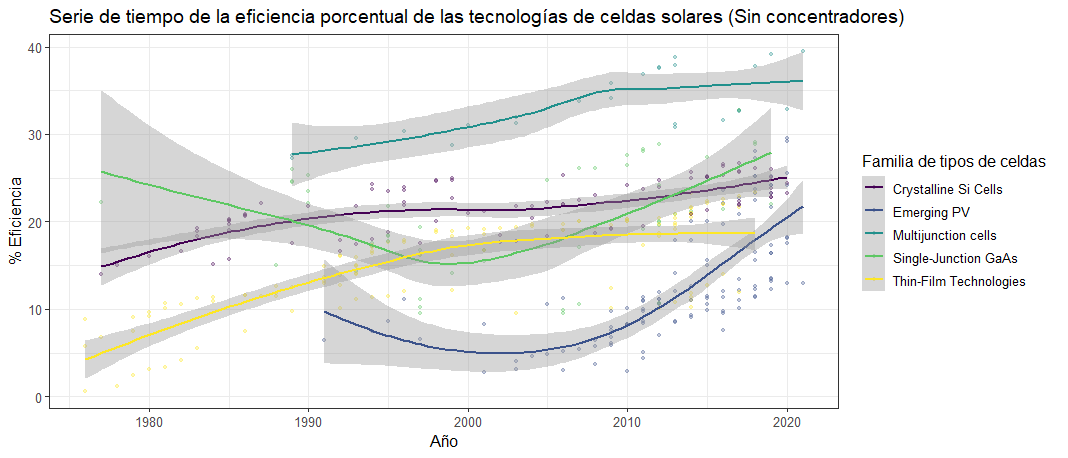
\includegraphics[scale=0.55]{img/SerieTiempo.png}
    \end{center}
    \caption{Serie de tiempo de las mejores eficiencias obtenidas en la investigación de las celdas solares según la agrupación dada por NREL.
    Fuente: \textit{National Renewable Energy Laboratory} \cite{nrel}}
    \label{img:SerieTiempo}
\end{figure}

Para contrastar dichas tecnlogías se pueden usar las mejores eficiencias de conversión energética de estos dispositivos obtenidos en el laboratorio que fueron recopilados por la NREL entre los años de 1980 y 2021 (Figura \ref{img:SerieTiempo}). En esa gráfica se observa que las tecnologías con mayor rendimiento han sido las celdas de unión múltiple, esto se debe a que sus arquitecturas fueron diseñadas para que haya un efecto sinérgico gracias a la apilación de los mejores materiales fotoeléctricos y de transporte de carga que existían en su época, no obstante, estos serían más costosos que los demás por la mayor cantidad y diversidad de materiales que se demandan para fabricarlos. También se aprecia que las tendencias de investigación de las celdas de silicio cristalino y las películas delgadas han desacelerado el aumento de sus rendimientos a diferencia de las celdas de unión simple Ga-As o emergentes. Es probable que esto sea consecuencia del descubrimiento de nuevos materiales con menores costos de producción, ambiental y con buen desempeño, por ejemplo: Moléculas orgánicas aceptoras-donadoras o \textit{quantum dots}.


Es un hecho que las tecnlogías emergentes están igualando, en términos de performance en el laboratorio, a las celdas comercialmente más comúnes como lo son las que se silicio multicristalino y las películas de Ga-As \cite{chowdhury2020overview}. Es por ello que es importante seguir investigándolas, pero como se mencionó anteriormente, esta familia reune diversas tecnologías y por tal motivo es importante sopesarlas desde el punto de vista de la sostenibilidad.

Con los datos del NREL se construyó una serie de tiempo de las mejores eficiencias que muestran en el laboratorio todos los tipos de celdas que pertenecen a las tecnologías emergentes  (Figura \ref{img:SerieEmergente}). En dicha gráfica se da cuenta que las celdas basadas en perovskitas encabezan a las demás y a su vez son las más recientes en ser exploradas, este material está compuesto por átomos de titanio y calcio dispuestos ortorrómbicamente cuando es cristalino, tiene un \textit{bandgap} de 1.5 eV, un alta constante dieléctrica, capacidad de separar rápidamente la carga y de ser funcionalizados con CIGS, Si, Sn y/o Pb para extender el rango de absorción del expectro solar (300-800 nm) y aumentar el coeficiente de absorción ($10^5cm^{-1}$) \cite{velilla2019outdoor}. A pesar de que estas ventajas han hecho de las celdas de perovskitas las más promisorias de las emergentes, la exposición al ambiente de estos dispositivos serían tóxico para la salud de los seres vivos, debido al Sn o Pb \cite{wang2022sustainable}. Otras celdas que presentan el mismo problema son las que tienen \textit{quantum dots}\cite{pan2014high} o compuestos inorgánicos CZTSSe\cite{suryawanshi2013czts}, ya contienen Cd y Sn respectivamente, aparte que hay esfuerzos por mejorar su estabilidad y disminuir sus costos de fabricación, los cuales dificultan su comercialización. 

Contrario a las ya mencionadas tecnologías emergentes, las celdas orgánicas y sensibilizadas por tintes son más sostenibles gracias a la capacidad de degradación de los polímeros que los componen, además tienen otras ventajas como es su fabricación modular que permite alternar 

\begin{figure}[h!]
    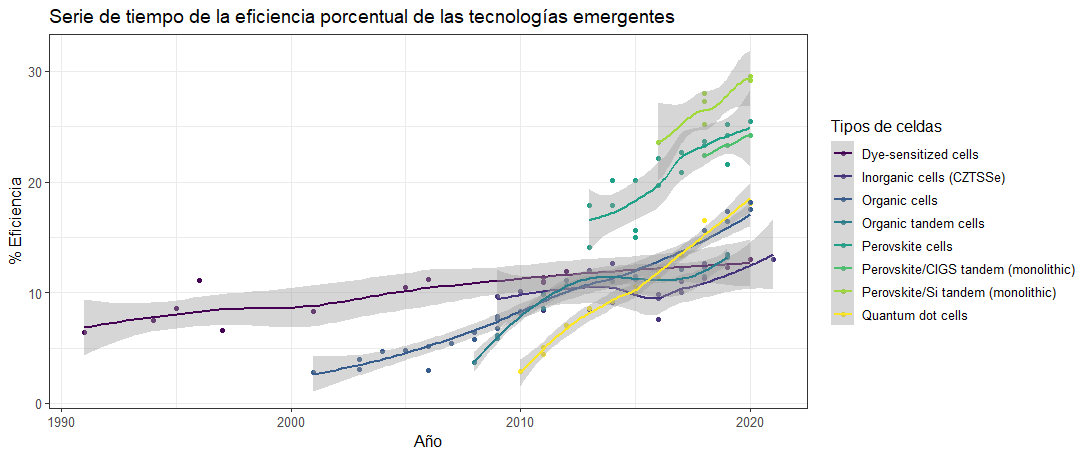
\includegraphics[scale=0.5]{img/SeriesEmergentes.png}
    \caption{Serie de tiempo de las mejores eficiencias obtenidas en la investigación de las tecnologías emergentes de celdas solares.
    Fuente: \textit{National Renewable Energy Laboratory} \cite{nrel}}
    \label{img:SerieEmergente}
\end{figure}


\begin{figure}[h!]
    \label{img:CSPT}
    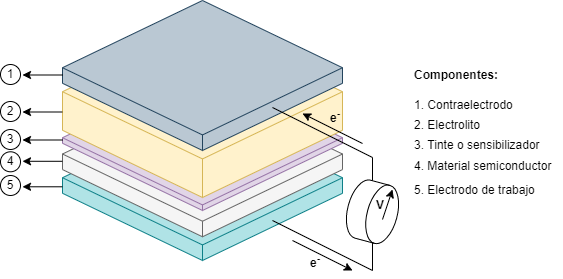
\includegraphics[scale=0.65]{img/DSSC.png}
    \caption{Serie de tiempo de las mejores eficiencias obtenidas en la investigación de las celdas solares según la agrupación dada por NREL.
    Fuente: \textit{National Renewable Energy Laboratory} \cite{owidenergy}}
\end{figure}


Finalmente, la tercera generación agrupa a las celdas más recientes tales como aquellas basadas en concentradores, nano cristales, polímeros y sensibilizadas por tintes. Las celdas por concentradores son dispositivos rígidos que aprovechan la radiación y el calor que se generan en al incidir luz en lentes convexos \cite{bertolli2008}, si bien tiene viabilidad comercial se demandan mejoras en los materiales fotovoltaicos. Las celdas basadas en nano cristales o \textit{quantum dots} (QD) pueden capturar mejor la luz mientras suprimen fenómenos de recombinación además de tener un rendimiento estable por encima del 20\% , no obstante no son comercialmente viables porque son costosos de fabricar \cite{jean2018synthesis}. Por el contrario, las celdas de polímero se caracterizan por su flexibilidad pero sus rendimientos estan en promedio por debajo del 10\% y a su vez son inestables porque son sensibles a cambios de temperatura y presión \cite{gusain2019polymer}. Por último, las celdas sensibilizadas por tintes son dispositivos que tienen semiconductores fotosensibilizados y ensamblados a un sistema electrolítico que permite un flujo continuo de electrones \cite{suhaimi2015materials}, se caracterizan por su construcción versátil y de bajo costo gracias a la diversidad materiales de sus componentes, sin embargo sus rendimientos aún no se equiparan a las comerciales de silicio \cite{sharma2018dye}. 


Las celdas sensibilizadas por tintes (CSPT) pueden ser 

$\dots$ debido a todas estas razones, la investigación de nuevos materiales y procesos de fabricación para celdas solares sensibilizadas por tintes más costo eficientes cobran relevancia. 


Las estructura de las celdas solares 


Es claro que deben de validarse experimentalmente los resultados obtenidos por los métodos compuacionales, pero estos pueden discriminar cientos de candidat


pero dado un grado de precisión razonable  en la predicción de la propiedad del material, estos modelos computcionales aceleran el proceso de elegir mejores estructuras o moléculas candidatas con la correcta combinación de propiedades necesarias para cumplir satisfactoriamente con el propósito para las que fueron hechas \textit{Leon R. Devereux}. 

\begin{figure}[h!]
    \begin{center}
        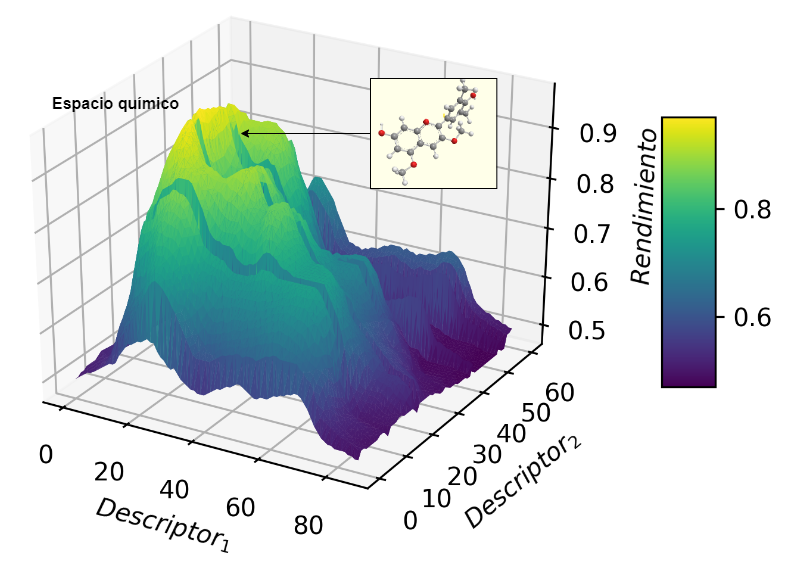
\includegraphics[scale=0.45]{img/espacioquimico.png}
    \end{center}
    \label{img:espacioquimico}
    \caption{Serie de tiempo de las mejores eficiencias obtenidas en la investigación de las celdas solares según la agrupación dada por NREL.
    Fuente: \textit{National Renewable Energy Laboratory} \cite{owidenergy}}
\end{figure}

\begin{figure}[h!]
    \begin{center}
        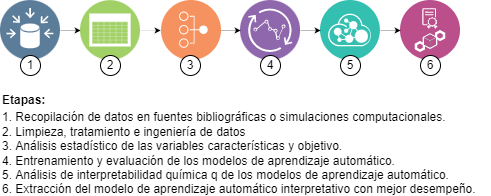
\includegraphics[scale=0.7]{img/etapas.png}
    \end{center}
    \label{img:etapas}
    \caption{Serie de tiempo de las mejores eficiencias obtenidas en la investigación de las celdas solares según la agrupación dada por NREL.
    Fuente: \textit{National Renewable Energy Laboratory} \cite{owidenergy}}
\end{figure}